%% ─── Sección 1 ──────────────────────────────────────────────────────────────
\section{Introducción}

\begin{frame}{Introducción}
    \begin{itemize}
        \item Los convertidores Boost son ampliamente usados en sistemas fotovoltaicos \cite{mohan2003}.
        \item El control MPPT maximiza la potencia extraída del panel solar.
        \item Este trabajo presenta el diseño y simulación del sistema.
    \end{itemize}
\end{frame}

%% ─── Sección 2 ──────────────────────────────────────────────────────────────
\section{Desarrollo}

\begin{frame}{Modelo Matemático}
    La tensión de salida del convertidor Boost es:
    \begin{equation}
        V_o = \frac{V_{in}}{1 - D}
    \end{equation}
    donde $D \in [0,1)$ es el ciclo de trabajo.

    \vspace{0.5em}
    \begin{block}{Modo de conducción continua}
        Se asume operación en modo continuo para el diseño nominal.
    \end{block}
\end{frame}

\begin{frame}{Tabla de Parámetros}
    \begin{table}
        \centering
        \begin{tabular}{lcc}
            \toprule
            Parámetro        & Símbolo   & Valor   \\
            \midrule
            Tensión entrada  & $V_{in}$  & 24 V    \\
            Inductancia      & $L$       & 1 mH    \\
            Capacitancia     & $C$       & 100 µF  \\
            Ciclo de trabajo & $D$       & 0.5     \\
            \bottomrule
        \end{tabular}
        \caption{Parámetros del convertidor Boost}
    \end{table}
\end{frame}

\begin{frame}{Gráfica de ejemplo}
    \begin{center}
        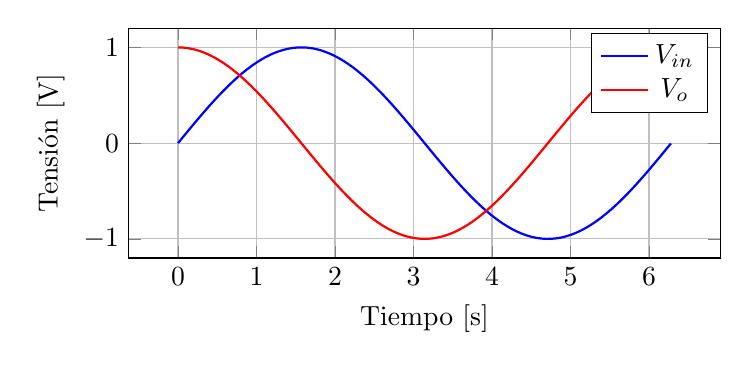
\begin{tikzpicture}
            \begin{axis}[
                xlabel={Tiempo [s]},
                ylabel={Tensión [V]},
                grid=major,
                width=0.75\textwidth,
                height=4.5cm,
            ]
                \addplot[blue, thick, domain=0:6.28, samples=100] {sin(deg(x))};
                \addplot[red,  thick, domain=0:6.28, samples=100] {cos(deg(x))};
                \legend{$V_{in}$, $V_o$}
            \end{axis}
        \end{tikzpicture}
    \end{center}
\end{frame}

%% ─── Sección 3 ──────────────────────────────────────────────────────────────
\section{Conclusiones}

\begin{frame}{Conclusiones}
    \begin{enumerate}
        \item El modelo matemático describe correctamente el comportamiento del convertidor.
        \item El control MPPT mejora la eficiencia del sistema fotovoltaico \cite{mppt2020}.
        \item El flujo con Tectonic + Beamer es compatible y reproducible.
    \end{enumerate}
\end{frame}